\chapter[Da variação à incerteza]{Da variação à incerteza: probabilidade, distribuições e associação}

No capítulo anterior, aprendemos a olhar para valores já observados. Calculamos centros, posições e dispersões para responder como uma turma, um processo ou um conjunto de atendimentos se comportou. Agora surge uma pergunta diferente: o que podemos dizer antes de conhecer o próximo resultado? Um painel informa que $20\%$ dos chamados anteriores foram reabertos; uma equipe quer estimar a chance de a próxima solicitação ser reaberta, a possibilidade de ocorrerem três reaberturas em dez chamados e a relação entre tempo de atendimento e satisfação. A estatística descritiva organiza o passado; a probabilidade cria uma linguagem disciplinada para raciocinar sob incerteza.

Essa linguagem não elimina o acaso e não transforma possibilidade em certeza. Ela especifica o conjunto de resultados possíveis, define quais resultados formam o evento de interesse e atribui números coerentes entre zero e um. Ao longo do capítulo, construiremos experimento aleatório, espaço amostral, evento, complemento, união, interseção, probabilidade condicional e independência. Usaremos tabelas e árvores pequenas para enxergar as relações antes de aplicar fórmulas.

Depois, uma variável aleatória transformará resultados em números e a esperança matemática expressará o valor médio de longo prazo. Distribuições discretas e contínuas organizarão as probabilidades possíveis. Bernoulli e binomial representarão tentativas com dois resultados; a uniforme representará resultados igualmente densos em um intervalo; e a normal introduzirá a conhecida forma de sino sem exigir cálculo integral. Cada modelo virá acompanhado das condições que justificam seu uso.

No fechamento, voltaremos aos dados observados e conectaremos duas variáveis. Covariância mostrará a direção em que elas variam juntas. A correlação de Pearson retirará o efeito das unidades e colocará a associação linear entre $-1$ e $1$. As contas serão realizadas linha a linha, com tabela de desvios, produtos e quadrados. A advertência de que associação não implica causalidade aparecerá dentro dessa explicação, no ponto em que ela se torna necessária, e não como um bloco desconectado.

O capítulo sustenta um encontro de três horas. Antes da chamada, percorremos a retomada da dispersão, a linguagem de eventos e as regras de combinação. Depois das 20h30, variáveis aleatórias e distribuições preparam a análise conjunta; a última parte calcula covariância e correlação. Não haverá código nem exercícios formais. Os pequenos casos resolvidos pertencem à narrativa do livro e servem para que turma e professor reconstruam juntos cada decisão matemática.

\begin{SummaryBox}
Então, aluno, veja só a mudança de perspectiva: antes resumimos aquilo que aconteceu; agora formalizaremos aquilo que pode acontecer e, ao final, mediremos como duas características observadas se movem juntas. A ponte entre os dois capítulos é a variação.
\end{SummaryBox}

\section{Da dispersão observada à incerteza sobre o próximo caso}

Retomemos uma pequena população de tempos, em minutos, ${8,10,10,12}$. Sua média populacional é
\[
\mu=\frac{8+10+10+12}{4}=\frac{40}{4}=10.
\]
Os desvios em relação à média são $-2,0,0,2$, e seus quadrados são $4,0,0,4$. A soma quadrática é $8$. Como descrevemos toda a população definida, dividimos por $N=4$:
\[
\sigma^2=\frac{8}{4}=2\text{ minutos}^2,
\qquad
\sigma=\sqrt{2}\approx1{,}41\text{ minuto}.
\]

A variância e o desvio-padrão descrevem o espalhamento do conjunto que conhecemos. A variância trabalha com desvios ao quadrado; o desvio-padrão retorna à unidade original. Entretanto, nenhum dos dois afirma exatamente qual será o tempo do próximo atendimento. Mesmo em um processo relativamente estável, o próximo caso pode levar oito, dez, doze ou outro número de minutos. A dispersão observada nos avisa que há variação; a probabilidade organiza nossa incerteza sobre resultados ainda não conhecidos.

A necessidade de raciocinar sobre acaso acompanha jogos, seguros, comércio, astronomia e decisões médicas há séculos. Problemas de jogos de azar ajudaram a formalizar a probabilidade nos séculos XVII e XVIII, mas a ideia se tornou muito mais ampla: estimar risco, comparar tratamentos, controlar qualidade e planejar capacidade. O objetivo não é prever individualmente com certeza. É estabelecer regras coerentes para comparar possibilidades e atualizar decisões quando recebemos informação.

Na interpretação clássica, resultados considerados igualmente possíveis permitem calcular probabilidade como razão entre casos favoráveis e casos possíveis. Em um dado honesto, a chance de obter um número par é $3/6=1/2$. Essa abordagem funciona quando a simetria justifica a igualdade. Na interpretação frequentista, a probabilidade descreve a frequência relativa que tende a se estabilizar em muitas repetições. Na interpretação subjetiva ou bayesiana, representa um grau de crença coerente diante da informação disponível. Neste capítulo, usaremos principalmente contagem e frequência, sempre declarando as condições.

Uma probabilidade $P(A)$ precisa satisfazer $0\leq P(A)\leq1$. Zero representa evento impossível no modelo; um, evento certo. Se todos os resultados possíveis formam o espaço $\Omega$, então $P(\Omega)=1$. Eventos mutuamente exclusivos podem ter probabilidades somadas. Esses princípios parecem simples, mas evitam contradições como atribuir $70\%$ de chance a um evento e $50\%$ a seu complemento.

O número não é mais forte do que o modelo. Dizer que há $20\%$ de chance de reabertura pode significar que vinte em cem casos comparáveis foram reabertos, mas o valor deixa de servir se mudarem produto, equipe, período ou definição de reabertura. Probabilidade não apaga contexto. Ela condiciona uma afirmação a um experimento e a premissas que precisam ser sustentadas.

Começaremos, portanto, não por uma fórmula, mas por três objetos: qual processo pode produzir um resultado, quais resultados consideramos possíveis e qual conjunto deles interessa à decisão. Esses objetos recebem os nomes experimento, espaço amostral e evento.

Há ainda uma distinção prática entre variabilidade e incerteza. Variabilidade é a diferença efetiva entre unidades ou repetições: alguns atendimentos duram mais do que outros. Incerteza é aquilo que não sabemos sobre um caso, uma média ou um mecanismo. Podemos ter grande variabilidade e pouca incerteza sobre a distribuição quando possuímos muitos dados estáveis; também podemos ter valores próximos entre si e grande incerteza porque observamos apenas duas unidades. A probabilidade será usada para representar mecanismos e incertezas declaradas, sem confundir a diferença que existe no mundo com a falta de informação de quem analisa.

\begin{SummaryBox}
Então, aluno, veja só o que você retomou: variância e desvio-padrão descrevem dispersão já observada. A probabilidade começa quando usamos um modelo para falar de resultados ainda incertos. O valor numérico só faz sentido junto das condições que definem o processo.
\end{SummaryBox}

\section{Experimento aleatório, espaço amostral e evento}

Um \textbf{experimento aleatório} é um procedimento cujo resultado não é conhecido antes da realização, embora o conjunto de possibilidades possa ser descrito. Lançar uma moeda, observar se um chamado será reaberto, medir o tempo da próxima consulta e selecionar uma matrícula são experimentos em sentidos diferentes. A palavra ``experimento'' não exige laboratório; exige uma regra que diga o que será realizado e qual observação encerrará a tentativa.

O \textbf{espaço amostral}, indicado por $\Omega$, reúne todos os resultados elementares considerados possíveis. Em um lançamento de dado,
\[
\Omega=\{1,2,3,4,5,6\}.
\]
Em um chamado classificado apenas como reaberto ou não reaberto,
\[
\Omega=\{R,N\}.
\]
Se medimos tempo, o espaço pode ser contínuo, como todos os valores reais não negativos. A qualidade do espaço depende do nível de detalhe da pergunta.

Um \textbf{evento} é um subconjunto de $\Omega$. No dado, o evento $A=$ ``resultado par'' é $A=\{2,4,6\}$. O evento $B=$ ``resultado maior que quatro'' é $B=\{5,6\}$. Cada resultado isolado também pode formar um evento, como $\{3\}$. O evento impossível é o conjunto vazio, $\emptyset$, e o evento certo é o próprio espaço amostral.

Quando os seis resultados do dado são igualmente prováveis, usamos
\[
P(A)=\frac{|A|}{|\Omega|}.
\]
$|A|$ é a quantidade de elementos favoráveis e $|\Omega|$ a quantidade total. Para $A=\{2,4,6\}$,
\[
P(A)=\frac{3}{6}=\frac{1}{2}=0{,}5=50\%.
\]
Para $B=\{5,6\}$,
\[
P(B)=\frac{2}{6}=\frac{1}{3}\approx0{,}333=33{,}3\%.
\]

Essa razão não deve ser aplicada mecanicamente. Em uma moeda deformada, cara e coroa podem não ter a mesma probabilidade. Em dados de atendimento, reaberto e não reaberto são duas categorias, mas não recebem automaticamente $1/2$ cada. Podemos estimar a chance pela frequência histórica: se $18$ de $120$ chamados comparáveis foram reabertos,
\[
\widehat{P}(R)=\frac{18}{120}=0{,}15=15\%.
\]
O chapéu indica estimativa obtida da amostra, não uma verdade exata e eterna.

O \textbf{complemento} de $A$, escrito $A^c$, reúne tudo que está em $\Omega$ e não pertence a $A$. Como $A$ e $A^c$ esgotam as possibilidades e não se sobrepõem,
\[
P(A^c)=1-P(A).
\]
Se $P(R)=0{,}15$, então
\[
P(R^c)=1-0{,}15=0{,}85=85\%.
\]
Interpretamos: no modelo e na população de referência, a chance de um chamado não ser reaberto é $85\%$.

O complemento é especialmente útil para eventos como ``ao menos um''. Muitas vezes é mais simples calcular a chance de nenhum caso e subtrair de um. Essa estratégia aparecerá na binomial. Antes, precisamos aprender a combinar eventos por união e interseção, distinguindo ``ou'' de ``e''.

Também é necessário distinguir resultado elementar de evento composto. No dado, o resultado $4$ é elementar porque corresponde a um único elemento de $\Omega$; ``par'' é composto porque reúne três resultados. Em um sistema, porém, o que parece elementar depende da representação: ``reaberto'' pode ocultar reabertura por falha técnica, informação incompleta ou mudança do cliente. Refinar o espaço amostral permite perguntas melhores, mas exige dados mais detalhados. Simplificá-lo facilita a conta, porém pode esconder diferenças decisivas. Assim, definir $\Omega$ já é uma escolha analítica.

\begin{GuidedBox}
Aluno, preste atenção aqui: duas categorias não significam duas chances iguais. A contagem de casos favoráveis sobre casos possíveis só vale diretamente quando os resultados elementares são equiprováveis. Em dados reais, a probabilidade precisa ser estimada ou sustentada por outro modelo.
\end{GuidedBox}

\begin{SummaryBox}
Então, aluno, veja só o que você aprendeu aqui: experimento define o procedimento; espaço amostral reúne os resultados possíveis; evento seleciona os resultados relevantes. O complemento contém tudo que não pertence ao evento e possui probabilidade $1-P(A)$.
\end{SummaryBox}

\section{União, interseção e probabilidade condicional}

Decisões reais combinam condições. Uma coordenação pode perguntar pela chance de um estudante ter baixa frequência \textit{ou} nota pendente; uma equipe pode investigar chamados urgentes \textit{e} reabertos. A \textbf{união} $A\cup B$ representa ``A ou B ou ambos''. A \textbf{interseção} $A\cap B$ representa ``A e B simultaneamente''. As palavras cotidianas podem ser ambíguas; os conjuntos tornam a relação explícita.

Para quaisquer eventos,
\[
P(A\cup B)=P(A)+P(B)-P(A\cap B).
\]
Subtraímos a interseção porque ela foi contada uma vez em $P(A)$ e outra em $P(B)$. No dado, $A=$ par $=\{2,4,6\}$ e $B=$ maior que quatro $=\{5,6\}$. A interseção é $A\cap B=\{6\}$; a união é $A\cup B=\{2,4,5,6\}$. Assim,
\[
P(A\cup B)=\frac{3}{6}+\frac{2}{6}-\frac{1}{6}=\frac{4}{6}=\frac{2}{3}.
\]

Se os eventos são mutuamente exclusivos, sua interseção é vazia. Em um único lançamento, ``obter 1'' e ``obter 6'' não podem ocorrer juntos, então $P(A\cap B)=0$ e a união é apenas a soma. Entretanto, ``par'' e ``maior que quatro'' não são exclusivos porque compartilham o $6$. Somar $3/6+2/6=5/6$ seria contar o resultado $6$ duas vezes.

A \textbf{probabilidade condicional} responde como a chance de $A$ muda quando sabemos que $B$ ocorreu:
\[
P(A\mid B)=\frac{P(A\cap B)}{P(B)},\qquad P(B)>0.
\]
O símbolo $\mid$ é lido ``dado que''. O denominador $P(B)$ mostra que restringimos o universo aos casos em $B$. Dentro desse novo universo, contamos quais também pertencem a $A$.

Considere uma turma de $40$ estudantes. Vinte e quatro trabalham durante o dia ($T$); dezesseis não trabalham. Doze dos que trabalham chegaram atrasados ($A$), e quatro dos que não trabalham chegaram atrasados. A tabela organiza as contagens:

\begin{center}
\small
\begin{tabular}{@{}lrrr@{}}
\toprule
 & \textbf{Atrasou $A$} & \textbf{Não atrasou $A^c$} & \textbf{Total} \\
\midrule
Trabalha $T$ & 12 & 12 & 24 \\
Não trabalha $T^c$ & 4 & 12 & 16 \\
\midrule
Total & 16 & 24 & 40 \\
\bottomrule
\end{tabular}
\end{center}

Sem condição, $P(A)=16/40=0{,}40$. Sabendo que o estudante trabalha, restringimos aos $24$ trabalhadores; entre eles, $12$ atrasaram:
\[
P(A\mid T)=\frac{12}{24}=0{,}50.
\]
Sabendo que não trabalha,
\[
P(A\mid T^c)=\frac{4}{16}=0{,}25.
\]
O resultado não afirma que trabalhar causa atraso; apenas descreve como a proporção observada muda entre os grupos.

Podemos reorganizar a fórmula condicional para obter a regra do produto:
\[
P(A\cap B)=P(A\mid B)P(B).
\]
No exemplo,
\[
P(A\cap T)=P(A\mid T)P(T)=\frac{12}{24}\times\frac{24}{40}=\frac{12}{40}=0{,}30.
\]
A conta acompanha uma sequência: selecionar um trabalhador e, dentro desse grupo, observar atraso.

A probabilidade condicional prepara a ideia de independência. Se conhecer $B$ não alterar a chance de $A$, os eventos são independentes. Se alterar, existe dependência probabilística no modelo. Precisamos distinguir essa definição de exclusão mútua, porque eventos impossíveis de ocorrer juntos quase nunca são independentes.

O sentido da condição também importa: $P(A\mid T)$ geralmente não é igual a $P(T\mid A)$. No exemplo, $P(A\mid T)=12/24=0{,}50$, enquanto $P(T\mid A)=12/16=0{,}75$. A primeira pergunta seleciona trabalhadores e procura atrasos; a segunda seleciona atrasados e procura trabalhadores. Numerador e denominador mudam porque o universo de referência mudou. Confundir as direções é comum em notícias sobre exames, riscos e classificadores. Antes de dividir, diga em voz alta qual grupo já é conhecido e qual característica será procurada dentro dele.

Vejamos um segundo exemplo resolvido, agora com um teste de triagem. Em mil atendimentos, cem pacientes possuem a condição investigada. O teste sinaliza positivo para noventa desses cem e também para noventa dos novecentos sem a condição. Assim, existem $180$ resultados positivos, dos quais apenas $90$ correspondem a pacientes com a condição. A sensibilidade é $P(+\mid D)=90/100=90\%$, mas a pergunta feita por quem recebeu o resultado é inversa: $P(D\mid +)=90/180=50\%$. O mesmo número $90$ aparece nos dois cálculos, porém os denominadores são diferentes porque as perguntas selecionam universos diferentes.

Esse caso funciona como contraexemplo para a intuição de que ``um teste com noventa por cento'' implica noventa por cento de chance após um positivo. A taxa básica da condição participa da interpretação. Se a condição fosse mais rara, os falsos positivos poderiam representar parcela ainda maior dos sinais; se fosse mais comum, a parcela de positivos verdadeiros aumentaria, mantendo as mesmas características do teste. Probabilidade condicional não é uma etiqueta permanente do evento: é uma relação entre evento, condição e população de referência.

Outro contraexemplo aparece quando trocamos ``ou'' por uma soma automática. Se $60\%$ dos estudantes usam transporte público e $50\%$ trabalham, não podemos concluir que $110\%$ usam transporte ou trabalham. Precisamos conhecer a interseção. Se $35\%$ fazem as duas coisas, então $P(T\cup W)=0{,}60+0{,}50-0{,}35=0{,}75$. Os $35\%$ foram contados nas duas parcelas e precisam ser retirados uma vez. O resultado final, $75\%$, responde à união inclusiva: transporte, trabalho ou ambos.

\begin{SummaryBox}
Então, aluno, veja só o que você aprendeu aqui: união é ``A ou B'', interseção é ``A e B''. Na união, retiramos a interseção contada duas vezes. Na condicional, reduzimos o universo aos casos em $B$ e observamos que parcela também está em $A$.
\end{SummaryBox}

\section{Independência, árvores de probabilidade e tabelas}

Dois eventos $A$ e $B$ são \textbf{independentes} quando saber que um ocorreu não altera a probabilidade do outro. Formalmente,
\[
P(A\mid B)=P(A),
\]
desde que $P(B)>0$. Uma forma equivalente é
\[
P(A\cap B)=P(A)P(B).
\]
A independência é uma propriedade a ser justificada pelo desenho do processo ou verificada no modelo; não deve ser presumida apenas para simplificar a conta.

Considere dois lançamentos de uma moeda honesta. O resultado do primeiro lançamento não altera o mecanismo do segundo. Se $C_1$ é cara no primeiro e $C_2$ é cara no segundo, $P(C_1)=1/2$ e $P(C_2)=1/2$. Pela independência,
\[
P(C_1\cap C_2)=\frac{1}{2}\times\frac{1}{2}=\frac{1}{4}.
\]
O espaço com sequências ${CC,CK,KC,KK}$ confirma quatro resultados equiprováveis, um deles com duas caras.

Eventos mutuamente exclusivos são diferentes. No mesmo lançamento, $A=$ cara e $B=$ coroa possuem $P(A\cap B)=0$, mas $P(A)P(B)=1/4$. Como $0\neq1/4$, não são independentes. Saber que saiu cara muda a chance de coroa para zero. Exclusão mútua significa que não ocorrem juntos; independência significa que a ocorrência de um não informa sobre o outro.

Uma árvore de probabilidade torna sequências visíveis. Suponha que $20\%$ dos chamados sejam urgentes ($U$). Entre urgentes, $30\%$ são reabertos ($R$); entre não urgentes, $10\%$ são reabertos. O primeiro nível possui $P(U)=0{,}20$ e $P(U^c)=0{,}80$. Do ramo $U$ saem $P(R\mid U)=0{,}30$ e $P(R^c\mid U)=0{,}70$. Do ramo $U^c$ saem $P(R\mid U^c)=0{,}10$ e $P(R^c\mid U^c)=0{,}90$.

A Figura~\ref{fig:arvore-urgencia} desenha exatamente esses dois estágios. Leia primeiro da esquerda para a direita: a primeira bifurcação separa urgência; a segunda usa probabilidades condicionais de reabertura dentro de cada ramo. Os valores nas folhas são probabilidades conjuntas, obtidas pela multiplicação ao longo do caminho.

\begin{figure}[htbp]
\centering
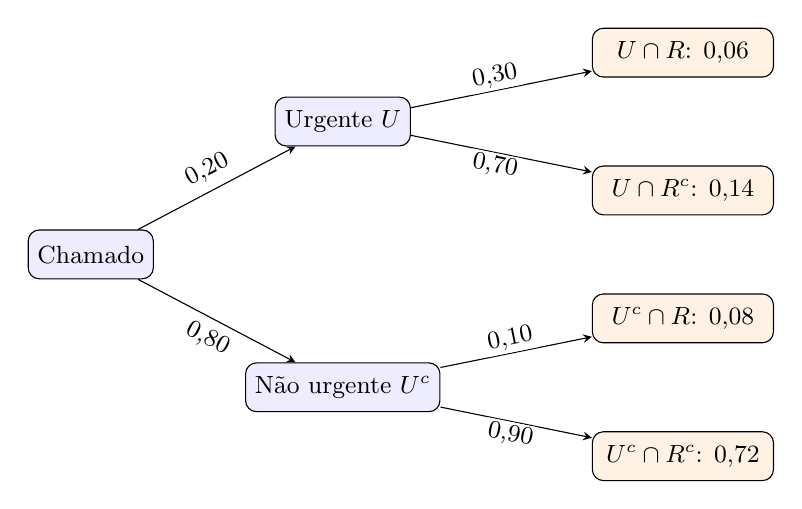
\begin{tikzpicture}[x=3.2cm,y=1.25cm,>=stealth,
every node/.style={font=\small},
state/.style={draw,rounded corners,fill=blue!7,minimum width=1.45cm,minimum height=.62cm,align=center},
leaf/.style={draw,rounded corners,fill=orange!10,minimum width=2.3cm,minimum height=.62cm,align=center}]
\node[state] (o) at (0,0) {Chamado};
\node[state] (u) at (1,1.35) {Urgente $U$};
\node[state] (n) at (1,-1.35) {Não urgente $U^c$};
\node[leaf] (ur) at (2.35,2.05) {$U\cap R$: $0{,}06$};
\node[leaf] (un) at (2.35,.65) {$U\cap R^c$: $0{,}14$};
\node[leaf] (nr) at (2.35,-.65) {$U^c\cap R$: $0{,}08$};
\node[leaf] (nn) at (2.35,-2.05) {$U^c\cap R^c$: $0{,}72$};
\draw[->] (o)--node[above,sloped] {$0{,}20$} (u);
\draw[->] (o)--node[below,sloped] {$0{,}80$} (n);
\draw[->] (u)--node[pos=.48,above,sloped,fill=white,inner sep=1pt] {$0{,}30$} (ur);
\draw[->] (u)--node[pos=.48,below,sloped,fill=white,inner sep=1pt] {$0{,}70$} (un);
\draw[->] (n)--node[pos=.48,above,sloped,fill=white,inner sep=1pt] {$0{,}10$} (nr);
\draw[->] (n)--node[pos=.48,below,sloped,fill=white,inner sep=1pt] {$0{,}90$} (nn);
\end{tikzpicture}
\caption{Árvore de urgência e reabertura: multiplicar ao longo de um caminho e somar caminhos que chegam ao mesmo evento.}
\label{fig:arvore-urgencia}
\end{figure}

Na Figura~\ref{fig:arvore-urgencia}, as duas folhas de reabertura somam $0{,}06+0{,}08=0{,}14$. Observe também que os ramos saindo de cada nó somam um: $0{,}30+0{,}70=1$ entre urgentes e $0{,}10+0{,}90=1$ entre não urgentes. Essa verificação simples encontra muitos erros de árvore. Não somamos $0{,}30$ com $0{,}10$ diretamente, pois são probabilidades definidas em grupos de tamanhos diferentes; primeiro ponderamos pelo tamanho probabilístico de cada ramo.

Multiplicamos ao longo de cada caminho. Para urgente e reaberto,
\[
P(U\cap R)=0{,}20\times0{,}30=0{,}06.
\]
Para não urgente e reaberto,
\[
P(U^c\cap R)=0{,}80\times0{,}10=0{,}08.
\]
Somamos caminhos alternativos que chegam a reabertura:
\[
P(R)=0{,}06+0{,}08=0{,}14.
\]
Portanto, a chance total de reabertura é $14\%$.

A mesma informação cabe em uma tabela de probabilidades conjuntas:

\begin{center}
\small
\begin{tabular}{@{}lrrr@{}}
\toprule
 & $R$ & $R^c$ & Total \\
\midrule
$U$ & 0,06 & 0,14 & 0,20 \\
$U^c$ & 0,08 & 0,72 & 0,80 \\
\midrule
Total & 0,14 & 0,86 & 1,00 \\
\bottomrule
\end{tabular}
\end{center}

Urgência e reabertura não são independentes, pois $P(R\mid U)=0{,}30$, enquanto $P(R)=0{,}14$. Conhecer urgência muda a chance estimada. Também podemos verificar pelo produto: $P(U)P(R)=0{,}20\times0{,}14=0{,}028$, diferente de $P(U\cap R)=0{,}06$. Isso mede dependência probabilística, mas ainda não explica o mecanismo. Chamados urgentes podem envolver problemas mais complexos, clientes diferentes ou critérios de registro distintos.

\begin{GuidedBox}
Aluno, preste atenção aqui: em árvore, multiplique ao seguir um caminho e some caminhos alternativos que formam o mesmo evento. A árvore mostra condicionais; a tabela mostra cruzamentos. As duas representações devem levar ao mesmo total.
\end{GuidedBox}

As árvores descrevem resultados categóricos. Para calcular médias esperadas de ganhos, custos, contagens ou tempos, precisamos atribuir um número a cada resultado. Essa função recebe o nome variável aleatória.

Em aplicações, independência pode ser razoável apenas condicionalmente. Resultados de estudantes da mesma turma compartilham professor e avaliação; chamados do mesmo cliente compartilham infraestrutura; medições sucessivas de uma máquina compartilham desgaste. Tratar essas unidades como tentativas independentes faz a quantidade de informação parecer maior do que realmente é. Uma árvore pequena ajuda a perguntar onde existe memória ou agrupamento. Quando a premissa não se sustenta, não ``consertamos'' a realidade para caber no produto das probabilidades; buscamos um modelo que represente a dependência.

Um exemplo numérico ajuda a testar a definição. Em um baralho comum, seja $A=$ ``carta vermelha'' e $B=$ ``carta de figura''. Temos $P(A)=26/52=1/2$, $P(B)=12/52=3/13$ e seis figuras vermelhas, portanto $P(A\cap B)=6/52=3/26$. O produto é $(1/2)(3/13)=3/26$, exatamente igual à interseção. Nesse modelo de uma carta, cor e condição de figura são independentes. Saber que a carta é vermelha não altera a proporção de figuras: continuam seis entre vinte e seis, ou $3/13$.

Agora mude o procedimento: retiramos duas cartas sem reposição e definimos $A=$ ``a primeira é ás'' e $B=$ ``a segunda é ás''. A chance inicial da segunda ser ás é $4/52$, por simetria. Contudo, se sabemos que a primeira foi ás, restam apenas três ases entre cinquenta e uma cartas, de modo que $P(B\mid A)=3/51$. Como $3/51\neq4/52$, os eventos não são independentes. A retirada sem reposição criou memória no processo. O contraexemplo mostra por que repetir uma fórmula de produto sem descrever reposição pode produzir uma resposta numericamente organizada e conceitualmente errada.

\begin{SummaryBox}
Então, aluno, veja só o que você aprendeu aqui: independência significa que a informação sobre um evento não muda a chance do outro. Em sequências, multiplicamos probabilidades condicionais ao longo de ramos e somamos caminhos que compõem o evento desejado.
\end{SummaryBox}

\section{Variável aleatória, esperança e variância probabilística}

Uma \textbf{variável aleatória} é uma função que associa um número real a cada resultado do experimento. O nome pode sugerir que a variável muda sem regra, mas a função é fixa; o acaso está em qual resultado ocorrerá. Em dois lançamentos de moeda, podemos definir $X=$ número de caras. As sequências $KK,CK,KC,CC$ recebem respectivamente os valores $0,1,1,2$. Assim, transformamos resultados em uma quantidade analisável.

Uma variável aleatória é \textbf{discreta} quando assume valores contáveis, como $0,1,2$ caras ou número de reaberturas. É \textbf{contínua} quando pode assumir qualquer valor em intervalos, como tempo e temperatura idealizados. A distinção muda a forma de atribuir probabilidade: na discreta, somamos massas em valores; na contínua, calculamos áreas em intervalos e a probabilidade de um ponto exato é zero no modelo.

A distribuição de probabilidade de $X$ informa a chance de cada valor. Para duas moedas honestas independentes,
\[
P(X=0)=\frac14,\qquad P(X=1)=\frac24=\frac12,\qquad P(X=2)=\frac14.
\]
As probabilidades são não negativas e somam um:
\[
\frac14+\frac12+\frac14=1.
\]
O valor $1$ possui maior probabilidade porque pode surgir por dois caminhos, $CK$ e $KC$.

A \textbf{esperança matemática} ou valor esperado é a média ponderada dos valores possíveis por suas probabilidades:
\[
E(X)=\sum_x xP(X=x).
\]
$x$ percorre os valores possíveis e $P(X=x)$ funciona como peso. Para o número de caras,
\[
E(X)=0\times\frac14+1\times\frac12+2\times\frac14
=0+\frac12+\frac12=1.
\]
Em muitas repetições de dois lançamentos, esperamos em média uma cara por par de lançamentos. Isso não significa que cada experimento produzirá uma cara.

O valor esperado atende à necessidade de planejar sob repetição. Considere um procedimento que economiza R\$ 20 com probabilidade $0{,}7$ e gera custo adicional de R\$ 10 com probabilidade $0{,}3$. Defina $G=20$ no primeiro caso e $G=-10$ no segundo. Então,
\[
E(G)=20\times0{,}7+(-10)\times0{,}3=14-3=11.
\]
O ganho esperado é R\$ 11 por ocorrência no modelo. Nenhuma ocorrência individual produz R\$ 11; os resultados possíveis continuam sendo R\$ 20 e R\$ $-10$.

Uma distribuição também possui variância:
\[
\operatorname{Var}(X)=E[(X-\mu_X)^2]
=\sum_x(x-\mu_X)^2P(X=x),
\]
em que $\mu_X=E(X)$. Para o número de caras, $\mu_X=1$. Calculamos
\[
\operatorname{Var}(X)=(0-1)^2\frac14+(1-1)^2\frac12+(2-1)^2\frac14
=\frac14+0+\frac14=\frac12.
\]
O desvio-padrão é $\sqrt{1/2}\approx0{,}707$ cara por experimento de dois lançamentos.

Esperança não basta para decidir entre alternativas com riscos distintos. Duas estratégias podem ter o mesmo ganho esperado e dispersões muito diferentes. Uma oferece ganho quase constante; outra alterna grande ganho e grande perda. A variância probabilística complementa a esperança assim como a variância descritiva complementou a média observada. A diferença é que agora ponderamos resultados possíveis pelas probabilidades do modelo.

Essa estrutura abre o caminho para distribuições nomeadas. Em vez de listar manualmente todas as probabilidades a cada problema, reconhecemos um mecanismo e usamos uma família matemática cujos parâmetros resumem as condições.

Uma transformação simples mostra por que a esperança é útil. Se cada reabertura custa R\$ 30, e $X$ conta reaberturas, então o custo é $C=30X$. Pela linearidade, $E(C)=30E(X)$. Se esperamos uma reabertura por lote, esperamos R\$ 30 de custo por lote, embora os custos reais possam ser R\$ 0, R\$ 30, R\$ 60 ou mais. A palavra ``esperado'' descreve média de longo prazo sob o modelo. Para orçamento, precisamos ainda da dispersão e de quantis, pois financiar apenas o valor médio pode ser insuficiente nos lotes desfavoráveis.

\begin{SummaryBox}
Então, aluno, veja só o que você aprendeu aqui: variável aleatória traduz resultados em números. Esperança é a média ponderada pelas probabilidades; variância probabilística mede o afastamento quadrático esperado. Nenhuma das duas promete o resultado de uma tentativa isolada.
\end{SummaryBox}

\section[Bernoulli e binomial]{Bernoulli e binomial: modelando tentativas com dois resultados}

A distribuição de \textbf{Bernoulli} representa uma única tentativa com dois resultados codificados como sucesso $1$ e insucesso $0$. ``Sucesso'' é apenas o evento de interesse, não um julgamento positivo. Em qualidade, sucesso pode significar defeito detectado; em atendimento, reabertura; em educação, entrega no prazo. O parâmetro $p$ é a probabilidade de $X=1$, e $1-p$ é a probabilidade de $X=0$.

Sua função de probabilidade pode ser escrita
\[
P(X=x)=p^x(1-p)^{1-x},\qquad x\in\{0,1\}.
\]
Se $x=1$, obtemos $p^1(1-p)^0=p$. Se $x=0$, obtemos $p^0(1-p)^1=1-p$. A fórmula reúne os dois casos. Para Bernoulli,
\[
E(X)=p,
\qquad
\operatorname{Var}(X)=p(1-p).
\]
Se a chance de reabertura é $0{,}2$, o indicador médio é $0{,}2$ e a variância é $0{,}2\times0{,}8=0{,}16$.

A distribuição \textbf{binomial} conta sucessos em $n$ tentativas Bernoulli. Ela exige um número fixo de tentativas, dois resultados por tentativa, probabilidade $p$ constante e independência entre tentativas. Se essas condições não forem razoáveis, a fórmula pode produzir um número preciso para um modelo inadequado. Por exemplo, chamados do mesmo cliente podem ser dependentes, e a taxa de reabertura pode mudar entre equipes.

Se $X$ é o número de sucessos, sua probabilidade é
\[
P(X=k)=\binom{n}{k}p^k(1-p)^{n-k},
\]
para $k=0,1,\ldots,n$. O coeficiente
\[
\binom{n}{k}=\frac{n!}{k!(n-k)!}
\]
conta quantas sequências diferentes possuem exatamente $k$ sucessos. O termo $p^k$ representa os sucessos; $(1-p)^{n-k}$, os insucessos.

Calculemos a chance de exatamente duas reaberturas em cinco chamados, assumindo independência e $p=0{,}2$. Primeiro, o número de maneiras de escolher duas posições entre cinco:
\[
\binom52=\frac{5!}{2!3!}
=\frac{5\times4\times3!}{(2\times1)3!}
=\frac{20}{2}=10.
\]
Depois,
\[
p^2=0{,}2^2=0{,}04,
\qquad
(1-p)^3=0{,}8^3=0{,}512.
\]
Multiplicamos:
\[
P(X=2)=10\times0{,}04\times0{,}512=0{,}2048.
\]
A chance modelada é $20{,}48\%$.

Para ``ao menos uma reabertura'', o complemento evita somar quatro casos. Calculamos nenhuma e subtraímos de um:
\[
P(X\geq1)=1-P(X=0).
\]
Como $\binom50=1$,
\[
P(X=0)=1\times0{,}2^0\times0{,}8^5=0{,}32768.
\]
Logo,
\[
P(X\geq1)=1-0{,}32768=0{,}67232=67{,}232\%.
\]
Uma chance individual de $20\%$ acumula-se em cinco oportunidades.

A Figura~\ref{fig:binomial-reaberturas} apresenta toda a distribuição desse mesmo caso. Cada haste representa $P(X=k)$ para $k=0,1,\ldots,5$. A figura permite comparar onde a massa se concentra e enxergar por que esperança igual a um não significa certeza de uma reabertura.

\begin{figure}[htbp]
\centering
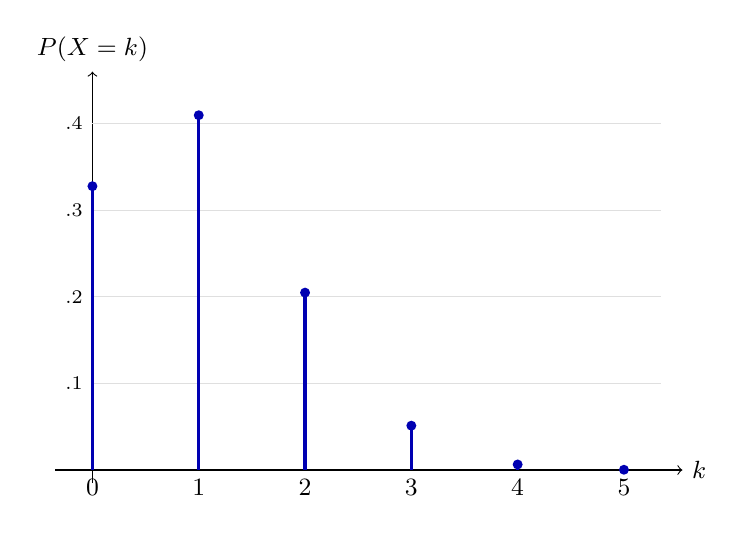
\begin{tikzpicture}[x=1.35cm,y=11cm,font=\small]
\draw[->] (-.35,0)--(5.55,0) node[right] {$k$};
\draw[->] (0,-.015)--(0,.46) node[above] {$P(X=k)$};
\foreach \y in {.1,.2,.3,.4}{\draw[gray!25] (0,\y)--(5.35,\y);\node[left,font=\scriptsize] at (0,\y) {\y};}
\foreach \x in {0,...,5}{\node[below] at (\x,0) {\x};}
\foreach \x/\p in {0/.32768,1/.40960,2/.20480,3/.05120,4/.00640,5/.00032}{\draw[very thick,blue!70!black] (\x,0)--(\x,\p);\fill[blue!70!black] (\x,\p) circle[radius=1.8pt];}
\end{tikzpicture}
\caption{Distribuição binomial para $n=5$ e $p=0{,}20$. A maior massa está em uma reabertura, mas outros totais continuam possíveis.}
\label{fig:binomial-reaberturas}
\end{figure}

Na Figura~\ref{fig:binomial-reaberturas}, $P(X=1)=5(0{,}2)(0{,}8)^4=0{,}4096$ é a haste mais alta. A probabilidade de zero, $0{,}32768$, ainda é considerável; exatamente duas possui $0{,}2048$; três ou mais concentram pouca massa. Somando todas as hastes obtemos um. Somando as hastes de um a cinco obtemos novamente $0{,}67232$, a probabilidade de ao menos uma calculada pelo complemento. A representação visual e a conta precisam concordar.

Considere agora outro exemplo resolvido: em oito entregas, a chance modelada de atraso é $p=0{,}10$. A probabilidade de exatamente dois atrasos é
\[
P(X=2)=\binom82(0{,}10)^2(0{,}90)^6=28\times0{,}01\times0{,}531441\approx0{,}1488.
\]
Portanto, sob as quatro premissas binomiais, cerca de $14{,}88\%$ dos lotes de oito teriam exatamente dois atrasos em repetição de longo prazo. O coeficiente $28$ não aumenta a chance arbitrariamente: ele conta as vinte e oito posições possíveis para os dois atrasos.

Como contraexemplo, imagine oito entregas realizadas pela mesma motocicleta durante uma tempestade que piora ao longo da noite. A chance de atraso não permanece constante, e um atraso inicial pode afetar os horários seguintes. Embora cada entrega possa ser rotulada atraso/não atraso e o total varie de zero a oito, a binomial deixa de representar adequadamente o mecanismo. Ter uma contagem inteira e dois rótulos é necessário, mas não suficiente. A pergunta correta deixa de ser ``qual número coloco em $p$?'' e passa a ser ``como represento dependência e mudança ao longo do tempo?''.

Na binomial,
\[
E(X)=np,
\qquad
\operatorname{Var}(X)=np(1-p).
\]
Para $n=5$ e $p=0{,}2$, $E(X)=5\times0{,}2=1$ reabertura e $\operatorname{Var}(X)=5\times0{,}2\times0{,}8=0{,}8$. O desvio-padrão é $\sqrt{0{,}8}\approx0{,}894$. Novamente, a esperança $1$ não afirma que cada lote terá exatamente uma reabertura.

\begin{GuidedBox}
Aluno, preste atenção aqui: binomial não significa apenas ``contar sim e não''. Verifique número fixo de tentativas, dois resultados, $p$ constante e independência. A fórmula deve ser consequência do mecanismo, não um molde escolhido porque os dados são inteiros.
\end{GuidedBox}

Bernoulli e binomial são discretas: atribuem massa a valores contáveis. Tempos e medidas pedem modelos contínuos. Começaremos por uma densidade constante, a uniforme, e depois veremos a forma de sino da normal.

O parâmetro $p$ merece atenção porque raramente é conhecido com exatidão. Se foi estimado por $20$ reaberturas em $100$ chamados, usamos $\hat p=0{,}20$ como aproximação. Outro período poderia gerar $18\%$ ou $23\%$. A probabilidade binomial calculada herda essa incerteza, além das premissas de constância e independência. Apresentar $20{,}48\%$ com muitas casas não torna a evidência mais precisa. A conta exata dentro do modelo e a adequação do modelo são perguntas diferentes, e ambas precisam aparecer na interpretação.

\begin{SummaryBox}
Então, aluno, veja só o que você aprendeu aqui: Bernoulli descreve uma tentativa com indicador $0/1$; binomial conta sucessos em $n$ tentativas sob condições explícitas. O coeficiente combinatório conta as posições possíveis dos sucessos.
\end{SummaryBox}

\section[Distribuições uniforme e normal]{Distribuições contínuas: uniforme e normal em linguagem introdutória}

Em uma variável contínua, probabilidades pertencem a intervalos. Uma densidade $f(x)$ deve ser não negativa e possuir área total igual a um. A probabilidade de $a\leq X\leq b$ é a área sob a curva entre $a$ e $b$. Como um ponto isolado tem largura zero, $P(X=x)=0$ no modelo contínuo, mesmo que valores arredondados apareçam repetidos em uma planilha.

Antes da curva teórica, precisamos olhar a forma observada. Um histograma divide uma variável quantitativa em intervalos, chamados classes ou \textit{bins}, e mostra em cada intervalo a contagem ou a frequência relativa. Diferentemente de um gráfico de barras categórico, as barras do histograma representam trechos contíguos do eixo numérico: a vizinhança entre $10$--$15$ e $15$--$20$ possui significado. A escolha das fronteiras e larguras resume os dados; não é uma fotografia ``exata'' e neutra da distribuição.

Considere tempos em minutos $4,5,6,7,8,9,10,11,12,13,20,21$. Com classes $[0,5)$, $[5,10)$, $[10,15)$, $[15,20)$ e $[20,25)$, as frequências são respectivamente $1,5,4,0,2$. A lacuna entre quinze e vinte e o pequeno grupo final ficam visíveis. Se usarmos apenas duas classes, $[0,12{,}5)$ e $[12{,}5,25)$, obtemos $9$ e $3$ e escondemos a lacuna. Se criarmos uma classe para cada minuto, a figura fica serrilhada e o padrão geral perde legibilidade. Poucos bins podem esconder estrutura; bins demais podem transformar variação amostral em ruído visual.

A Figura~\ref{fig:histograma-bins} mostra as duas primeiras escolhas para os mesmos dados. Observe que nenhum valor mudou. Mudou apenas a discretização usada para resumir a forma. A leitura responsável informa limites das classes, contagem ou densidade no eixo vertical e tamanho da amostra.

\begin{figure}[htbp]
\centering
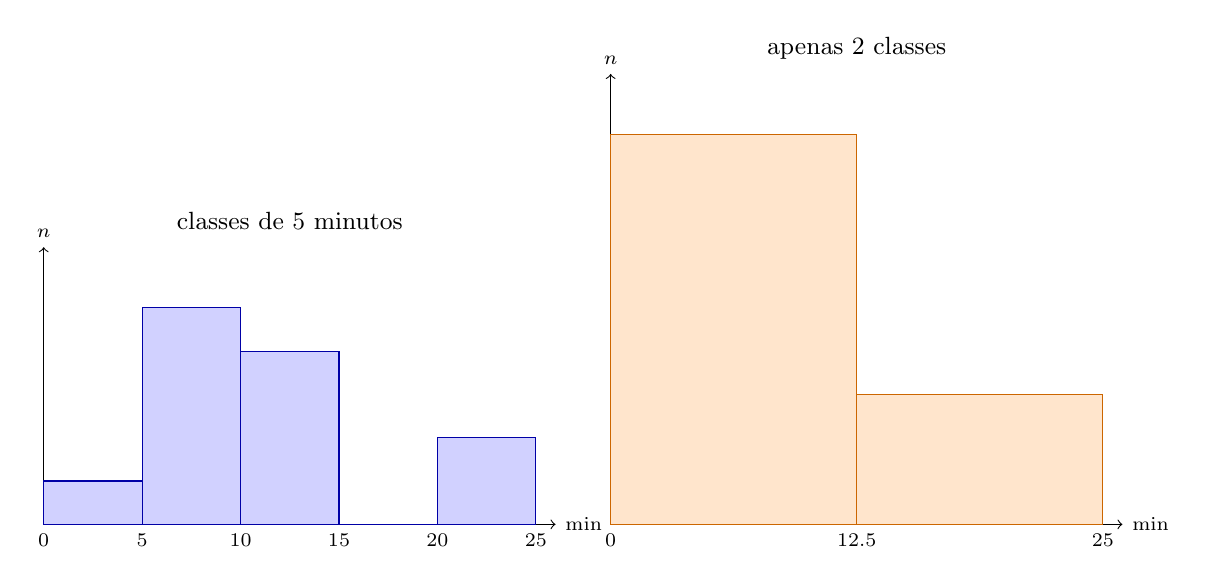
\begin{tikzpicture}[x=.25cm,y=.55cm,font=\scriptsize]
\begin{scope}
\draw[->] (0,0)--(26,0) node[right] {min};\draw[->] (0,0)--(0,6.4) node[above] {$n$};
\node[font=\small] at (12.5,7.0) {classes de 5 minutos};
\foreach \x/\w/\h in {0/5/1,5/5/5,10/5/4,15/5/0,20/5/2}{\draw[fill=blue!18,draw=blue!65!black] (\x,0) rectangle ++(\w,\h);}
\foreach \x in {0,5,10,15,20,25}{\node[below] at (\x,0) {\x};}
\end{scope}
\begin{scope}[xshift=7.2cm]
\draw[->] (0,0)--(26,0) node[right] {min};\draw[->] (0,0)--(0,10.4) node[above] {$n$};
\node[font=\small] at (12.5,11.0) {apenas 2 classes};
\draw[fill=orange!20,draw=orange!80!black] (0,0) rectangle (12.5,9);
\draw[fill=orange!20,draw=orange!80!black] (12.5,0) rectangle (25,3);
\foreach \x in {0,12.5,25}{\node[below] at (\x,0) {\x};}
\end{scope}
\end{tikzpicture}
\caption{Os mesmos tempos em histogramas com bins diferentes. A discretização altera o padrão visível, não os dados originais.}
\label{fig:histograma-bins}
\end{figure}

Na Figura~\ref{fig:histograma-bins}, a escolha de cinco minutos revela cauda e lacuna; a escolha grosseira resume apenas concentração geral. Uma heurística como $k\approx1+3{,}3\log_{10}(n)$ pode sugerir um ponto inicial para a quantidade de classes, mas não escolhe automaticamente a melhor representação. Precisamos comparar alternativas, manter escalas honestas e perguntar que estrutura permanece estável. Uma forma aproximadamente simétrica sem extremos costuma ser bem resumida por média e desvio-padrão; assimetria ou extremos pedem também mediana e IQR; duas modas convidam a investigar subgrupos.

A distribuição \textbf{uniforme contínua} representa densidade constante no intervalo $[a,b]$. Sua função é
\[
f(x)=\frac{1}{b-a},\qquad a\leq x\leq b,
\]
e zero fora. O denominador $b-a$ é a largura total; multiplicar altura $1/(b-a)$ pela largura produz área um. A probabilidade de um subintervalo é sua largura dividida pela largura total.

Suponha que um instante de chegada seja modelado uniformemente entre $0$ e $20$ minutos. Então $a=0$, $b=20$ e $f(x)=1/20=0{,}05$. A chance de chegar entre $5$ e $9$ minutos é
\[
P(5\leq X\leq9)=\frac{9-5}{20-0}=\frac4{20}=0{,}20.
\]
O resultado de $20\%$ vem da faixa de quatro minutos dentro de uma janela de vinte. Essa uniformidade precisa ser justificável; horários reais frequentemente concentram chegadas.

Para a uniforme,
\[
E(X)=\frac{a+b}{2},
\qquad
\operatorname{Var}(X)=\frac{(b-a)^2}{12}.
\]
No intervalo $[0,20]$, a esperança é $(0+20)/2=10$ minutos. A variância é $20^2/12=400/12\approx33{,}33$ minutos$^2$, e o desvio-padrão é $\sqrt{33{,}33}\approx5{,}77$ minutos. A simetria coloca o centro exatamente no ponto médio.

A distribuição \textbf{normal} surgiu no estudo de erros de medição e foi conectada aos trabalhos de De Moivre, Laplace e Gauss. Sua forma simétrica de sino tornou-se central porque muitos efeitos pequenos e aproximadamente independentes podem produzir somas próximas da normal. A normal é definida por média $\mu$ e desvio-padrão $\sigma$. A média determina o centro; o desvio-padrão determina a abertura.

Sua densidade é
\[
f(x)=\frac{1}{\sigma\sqrt{2\pi}}
\exp\left[-\frac{(x-\mu)^2}{2\sigma^2}\right].
\]
Não precisamos calcular exponenciais manualmente nesta introdução. Precisamos ler os símbolos: $x-\mu$ é a distância ao centro; o quadrado torna a curva simétrica; $\sigma^2$ controla como essa distância é escalada; e o fator frontal garante área total um. Aproximadamente $68\%$ da área fica entre $\mu-\sigma$ e $\mu+\sigma$, $95\%$ entre $\mu-2\sigma$ e $\mu+2\sigma$, em uma normal ideal.

O escore padronizado
\[
z=\frac{x-\mu}{\sigma}
\]
informa quantos desvios-padrão um valor está acima ou abaixo da média. Se tempos forem aproximadamente normais com $\mu=50$ e $\sigma=5$, um tempo $x=60$ tem
\[
z=\frac{60-50}{5}=\frac{10}{5}=2.
\]
Ele está dois desvios-padrão acima da média. Um tempo $45$ tem $z=(45-50)/5=-1$, um desvio abaixo.

A Figura~\ref{fig:normais-media-dp} separa os papéis de média e desvio-padrão. No painel esquerdo, as curvas possuem o mesmo $\sigma$ e centros diferentes; no direito, possuem a mesma média, mas dispersões diferentes. Antes de olhar os eixos, antecipe: mudar $\mu$ desloca o sino; aumentar $\sigma$ espalha a mesma área total e reduz a altura do pico.

\begin{figure}[htbp]
\centering
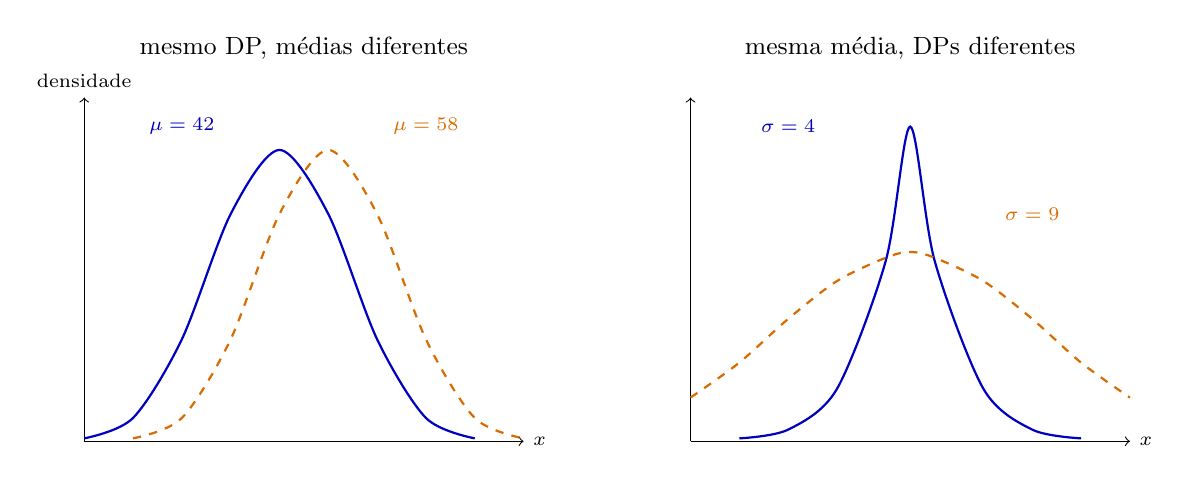
\begin{tikzpicture}[x=.62cm,y=3.7cm,font=\scriptsize]
\begin{scope}
\draw[->] (0,0)--(9,0) node[right] {$x$};\draw[->] (0,0)--(0,1.18) node[above] {densidade};
\node[font=\small] at (4.5,1.35) {mesmo DP, médias diferentes};
\draw[blue!75!black,thick,smooth] plot coordinates {(0,.01)(1,.08)(2,.35)(3,.78)(4,1)(5,.78)(6,.35)(7,.08)(8,.01)};
\draw[orange!85!black,thick,dashed,smooth] plot coordinates {(1,.01)(2,.08)(3,.35)(4,.78)(5,1)(6,.78)(7,.35)(8,.08)(9,.01)};
\node[blue!75!black] at (2.0,1.08) {$\mu=42$};\node[orange!85!black] at (7.0,1.08) {$\mu=58$};
\end{scope}
\begin{scope}[xshift=7.7cm]
\draw[->] (0,0)--(9,0) node[right] {$x$};\draw[->] (0,0)--(0,1.18);
\node[font=\small] at (4.5,1.35) {mesma média, DPs diferentes};
\draw[blue!75!black,thick,smooth] plot coordinates {(1,.01)(2,.04)(3,.18)(4,.62)(4.5,1.08)(5,.62)(6,.18)(7,.04)(8,.01)};
\draw[orange!85!black,thick,dashed,smooth] plot coordinates {(0,.15)(1,.27)(2,.42)(3,.55)(4,.63)(4.5,.65)(5,.63)(6,.55)(7,.42)(8,.27)(9,.15)};
\node[blue!75!black] at (2.0,1.08) {$\sigma=4$};\node[orange!85!black] at (7.0,.78) {$\sigma=9$};
\end{scope}
\end{tikzpicture}
\caption{A média desloca a normal; o desvio-padrão controla sua abertura. Todas as curvas preservam área total igual a um.}
\label{fig:normais-media-dp}
\end{figure}

No painel esquerdo da Figura~\ref{fig:normais-media-dp}, os dois processos possuem a mesma variabilidade modelada, mas níveis típicos diferentes. No painel direito, os centros coincidem, porém a curva com $\sigma=9$ atribui mais densidade às regiões afastadas. Ela fica mais baixa porque a área total continua sendo um. Uma curva mais alta não representa ``mais casos'' quando comparamos densidades normalizadas; representa maior concentração por unidade do eixo horizontal.

Para completar a leitura de $z$, suponha notas aproximadamente normais com média $70$ e desvio-padrão $8$. Uma nota $86$ possui $z=(86-70)/8=2$; uma nota $62$ possui $z=-1$. Esses escores permitem comparar posições relativas em escalas diferentes. Se outra prova tem média $500$ e desvio $50$, a pontuação $600$ também está a dois desvios acima do centro. O escore padroniza posição; não torna provas automaticamente equivalentes em conteúdo, dificuldade ou finalidade.

Aproximando pela regra $68$--$95$, cerca de $95\%$ dos valores do primeiro exemplo normal ideal estariam entre $70-2(8)=54$ e $70+2(8)=86$. Isso não significa que exatamente $95$ de cada grupo de cem cairão no intervalo, nem que valores externos sejam erros. Significa que o modelo atribui aproximadamente $5\%$ da área total às duas caudas, cerca de $2{,}5\%$ em cada uma pela simetria. Em uma amostra pequena, a proporção observada pode diferir.

Um contraexemplo esclarece o limite: tempos de espera com muitas observações curtas e poucos casos extremamente longos costumam formar cauda à direita. Aplicar a normal apenas porque conhecemos média e desvio-padrão pode atribuir probabilidade a tempos negativos e subestimar casos extremos. A curva deve responder ao mecanismo e à forma observada. O escore $z$ continua sendo uma padronização algébrica possível, mas a interpretação de áreas normais exige a hipótese adicional de distribuição aproximadamente normal.

Nem toda variável contínua é normal. Renda, tempo de espera e falhas podem ser assimétricos; dados limitados podem se acumular nas fronteiras; misturas de grupos podem gerar duas modas. Média e desvio-padrão não provam normalidade. Precisamos observar forma, processo e tamanho da amostra. A distribuição é um modelo útil quando suas implicações combinam com o fenômeno, não uma obrigação imposta pelo formato numérico.

Uniforme e normal também expressam incertezas diferentes. A uniforme declara a mesma densidade em todo o intervalo e fronteiras rígidas: fora de $[a,b]$, a probabilidade é zero. A normal concentra densidade perto de $\mu$ e possui caudas que, matematicamente, se estendem sem fronteira. Isso pode ser inadequado para variáveis impossíveis de serem negativas, sobretudo quando a média está perto de zero. Escolher distribuição significa comparar suporte, simetria, caudas e mecanismo, não apenas aproximar uma curva que pareça bonita sobre um histograma.

\begin{SummaryBox}
Então, aluno, veja só o que você aprendeu aqui: na uniforme, intervalos de mesma largura possuem a mesma probabilidade. Na normal, a média localiza o sino e o desvio-padrão controla sua abertura. Ambas são modelos contínuos e precisam ser justificadas pelo processo.
\end{SummaryBox}

\section{Covariância: quando duas variáveis se afastam juntas}

Até agora, estudamos uma variável ou eventos combinados. Na análise exploratória, frequentemente perguntamos se duas quantidades variam juntas: mais horas de estudo acompanham notas maiores? maior tempo de espera acompanha satisfação menor? A covariância surgiu para resumir a direção dessa variação conjunta. Ela compara o sinal do desvio de $X$ com o sinal do desvio correspondente de $Y$.

Antes de multiplicar desvios, desenhe ou leia a dispersão. O roteiro visual possui seis perguntas: qual direção predomina; quão apertados estão os pontos; a forma é aproximadamente linear ou curva; existem grupos separados; há observação influente; e uma terceira variável poderia explicar estratos diferentes? Esse checklist impede que a fórmula receba uma responsabilidade que não possui. Covariância resume direção líquida; ela não identifica sozinha curvatura, clusters ou erro de junção.

A galeria da Figura~\ref{fig:paineis-correlacao}, apresentada adiante junto de Pearson, deve ser antecipada mentalmente aqui: produtos cruzados serão positivos nos quadrantes em que os dois desvios compartilham sinal e negativos quando possuem sinais opostos. Numa nuvem crescente, positivos tendem a dominar; numa decrescente, negativos. Numa curva em U simétrica, os sinais podem cancelar-se apesar de uma relação nítida. A conta nasce dessa geometria centrada nas médias.

Para uma amostra de pares $(x_i,y_i)$, a covariância amostral é
\[
s_{XY}=\operatorname{Cov}(X,Y)=
\frac{1}{n-1}\sum_{i=1}^{n}(x_i-\bar{x})(y_i-\bar{y}).
\]
$n$ é a quantidade de pares; $\bar{x}$ e $\bar{y}$ são as médias; cada produto combina os desvios do mesmo caso. Se ambos são positivos ou ambos negativos, o produto é positivo. Se têm sinais opostos, o produto é negativo.

Use os pares horas de estudo e nota $(1,2)$, $(2,4)$, $(3,5)$, $(4,4)$ e $(5,10)$. Primeiro calculamos
\[
\bar{x}=\frac{1+2+3+4+5}{5}=\frac{15}{5}=3,
\]
\[
\bar{y}=\frac{2+4+5+4+10}{5}=\frac{25}{5}=5.
\]
Em seguida, abrimos desvios, produtos e quadrados na tabela.

\begin{center}
\small
\begin{tabular}{@{}rrrrrrr@{}}
\toprule
$x_i$ & $y_i$ & $x_i-3$ & $y_i-5$ & Produto & $(x_i-3)^2$ & $(y_i-5)^2$ \\
\midrule
1 & 2  & $-2$ & $-3$ & 6  & 4 & 9 \\
2 & 4  & $-1$ & $-1$ & 1  & 1 & 1 \\
3 & 5  & 0    & 0    & 0  & 0 & 0 \\
4 & 4  & 1    & $-1$ & $-1$ & 1 & 1 \\
5 & 10 & 2    & 5    & 10 & 4 & 25 \\
\midrule
 & & 0 & 0 & 16 & 10 & 36 \\
\bottomrule
\end{tabular}
\end{center}

A soma dos produtos centrados é $6+1+0-1+10=16$. Como tratamos os cinco pares como amostra,
\[
s_{XY}=\frac{16}{5-1}=\frac{16}{4}=4.
\]
A covariância positiva indica que valores de $X$ acima de sua média tendem a acompanhar valores de $Y$ acima da média, e valores abaixo tendem a acompanhar valores abaixo. O par $(4,4)$ produz $-1$ porque estudo está acima da média e nota abaixo.

Se os produtos negativos dominassem, a covariância seria negativa: quando uma variável estivesse acima do centro, a outra tenderia a ficar abaixo. Uma covariância próxima de zero indicaria ausência de variação conjunta linear evidente, mas poderia esconder relações curvas ou grupos diferentes. O sinal é informativo; a magnitude depende das unidades.

Neste exemplo, horas multiplicadas por pontos formam a unidade da covariância. Se horas forem convertidas em minutos, todos os desvios de $X$ serão multiplicados por $60$ e a covariância também. O fenômeno não mudou, mas o número mudou de escala. Para comparar relações em unidades diferentes, precisamos padronizar a covariância pelos desvios-padrão.

Façamos um exemplo resolvido com direção negativa. Considere tempo de espera $X=(1,2,3,4)$ e satisfação $Y=(10,8,6,4)$. As médias são $\bar{x}=2{,}5$ e $\bar{y}=7$. Os desvios de $X$ são $(-1{,}5,-0{,}5,0{,}5,1{,}5)$; os de $Y$ são $(3,1,-1,-3)$. Os produtos correspondentes são $-4{,}5$, $-0{,}5$, $-0{,}5$ e $-4{,}5$, cuja soma é $-10$. Logo,
\[
s_{XY}=\frac{-10}{4-1}=-\frac{10}{3}\approx-3{,}33.
\]
O sinal negativo aparece porque esperas abaixo da média acompanham satisfações acima da média e vice-versa. A unidade é minuto vezes ponto de satisfação.

Agora compare um conjunto com produtos que se cancelam. Para $X=(-2,-1,1,2)$ e $Y=(4,1,1,4)$, ambas as médias já são $0$ e $2{,}5$, respectivamente. Os produtos centrados são $(-2)(1{,}5)=-3$, $(-1)(-1{,}5)=1{,}5$, $(1)(-1{,}5)=-1{,}5$ e $(2)(1{,}5)=3$. A soma é zero, então a covariância é zero. Contudo, $Y$ depende claramente de $|X|$: valores extremos de $X$ acompanham valores altos de $Y$. Este contraexemplo mostra que covariância zero não significa ausência de relação; significa ausência de movimento conjunto linear líquido nesse arranjo.

Também podemos enxergar por que deslocar a origem não muda a covariância. Se somarmos cem a todos os valores de $X$, a nova média também aumenta cem e cada desvio $x_i-\bar{x}$ permanece igual. Já multiplicar $X$ por sessenta multiplica seus desvios e a covariância por sessenta. Assim, a covariância ignora a escolha do zero, mas não é imune à escolha da unidade. Essa propriedade prepara a normalização feita por Pearson.

A ordem dos pares jamais pode ser perdida. Se ordenarmos separadamente as horas e as notas, fabricaremos correspondências que não pertencem aos estudantes observados e provavelmente aumentaremos a covariância. Cada produto $(x_i-\bar{x})(y_i-\bar{y})$ deve usar as duas características da mesma unidade. Essa exigência conecta estatística à qualidade dos dados: identificadores, junções e granularidade determinam se os pares representam relações reais ou combinações acidentais. Antes da fórmula, confira que uma linha corresponde a uma unidade coerente.

\begin{SummaryBox}
Então, aluno, veja só o que você aprendeu aqui: covariância multiplica desvios correspondentes. Produtos positivos indicam movimento no mesmo sentido; negativos, sentidos opostos. Sua escala depende das unidades, por isso ela prepara, mas não encerra, a medida de associação.
\end{SummaryBox}

\section{Correlação de Pearson e a síntese da associação linear}

A correlação de Pearson, associada ao desenvolvimento da estatística moderna no fim do século XIX, padroniza a covariância pelos desvios-padrão de $X$ e $Y$:
\[
r=\frac{s_{XY}}{s_Xs_Y}.
\]
$r$ é a correlação amostral; $s_{XY}$ é a covariância amostral; $s_X$ e $s_Y$ são os desvios-padrão amostrais. O resultado fica entre $-1$ e $1$. O sinal indica direção e o valor absoluto indica força da associação linear.

Usaremos as somas da tabela. Para $X$, a soma quadrática é $10$:
\[
s_X^2=\frac{10}{5-1}=\frac{10}{4}=2{,}5,
\qquad
s_X=\sqrt{2{,}5}\approx1{,}581.
\]
Para $Y$, a soma quadrática é $36$:
\[
s_Y^2=\frac{36}{4}=9,
\qquad
s_Y=\sqrt9=3.
\]
Já obtivemos $s_{XY}=4$.

Substituímos na fórmula:
\[
r=\frac{4}{(1{,}581)(3)}
=\frac{4}{4{,}743}
\approx0{,}843.
\]
O valor indica associação linear positiva forte neste pequeno conjunto: maiores horas tendem a acompanhar maiores notas. A palavra ``tendem'' preserva a variação; o par $(4,4)$ mostra que a relação não é perfeita.

Podemos obter o mesmo resultado diretamente das somas centradas:
\[
r=\frac{\sum(x_i-\bar{x})(y_i-\bar{y})}
{\sqrt{\sum(x_i-\bar{x})^2\sum(y_i-\bar{y})^2}}
=\frac{16}{\sqrt{10\times36}}
=\frac{16}{\sqrt{360}}
\approx\frac{16}{18{,}974}
\approx0{,}843.
\]
Os divisores $n-1$ se cancelam porque aparecem na covariância e nos dois desvios.

Uma correlação $r=1$ representa pares exatamente sobre uma reta crescente; $r=-1$, sobre uma reta decrescente; $r$ próximo de zero indica pouca associação \textit{linear}. A palavra linear é indispensável. Se $Y=X^2$ e $X$ assume valores simétricos negativos e positivos, a relação é perfeitamente determinada e curva, mas Pearson pode ficar próximo de zero. Um gráfico de dispersão deve acompanhar a correlação para revelar forma, grupos e pontos influentes.

A Figura~\ref{fig:paineis-correlacao} coloca quatro situações lado a lado: tendência positiva, tendência negativa, relação não linear e conjunto dominado por um ponto influente. A intenção não é estimar o coeficiente apenas pela aparência, mas aprender quais perguntas o coeficiente isolado não responde.

\begin{figure}[htbp]
\centering
\begin{tikzpicture}[x=.52cm,y=.30cm,font=\scriptsize]
\newcommand{\panelaxes}[1]{\draw[gray!35] (-3,0)--(3,0);\draw[gray!35] (0,-3)--(0,10);\draw (-3,-3) rectangle (3,10);\node[font=\small] at (0,11) {#1};}
\begin{scope}\panelaxes{positiva linear}\foreach \x/\y in {-2/-2.2,-1.5/-1,-.5/-.8,.2/.5,1/1.1,1.8/2.4,2.5/2.2}{\fill[blue!75!black] (\x,\y) circle[radius=2.2pt];}\end{scope}
\begin{scope}[xshift=7.0cm]\panelaxes{negativa linear}\foreach \x/\y in {-2/2.4,-1.4/1.2,-.7/1,0/.1,.8/-1.1,1.6/-1.4,2.5/-2.6}{\fill[orange!85!black] (\x,\y) rectangle ++(.14,.24);}\end{scope}
\begin{scope}[yshift=-5.1cm]\panelaxes{não linear: $Y=X^2$}\foreach \x/\y in {-3/9,-2/4,-1/1,0/0,1/1,2/4,3/9}{\fill[blue!75!black] (\x,\y) circle[radius=2.2pt];}\end{scope}
\begin{scope}[xshift=7.0cm,yshift=-5.1cm]\panelaxes{um ponto influente}\foreach \x/\y in {-2/.2,-1.5/-.1,-1/.1,-.5/0,0/.2,.5/-.2,3/9}{\fill[orange!85!black] (\x,\y) circle[radius=2.2pt];}\end{scope}
\end{tikzpicture}
\caption{Quatro dispersões que exigem ler forma, direção e influência antes de resumir com Pearson.}
\label{fig:paineis-correlacao}
\end{figure}

Nos dois painéis superiores da Figura~\ref{fig:paineis-correlacao}, uma reta resume razoavelmente a direção, positiva ou negativa. No painel inferior esquerdo, há relação perfeita e previsível, mas simétrica e curva; produtos positivos e negativos podem cancelar-se, deixando $r$ próximo de zero. No inferior direito, seis pontos formam uma nuvem quase horizontal, enquanto um único ponto distante cria uma tendência positiva aparente. Portanto, sempre associe $r$ ao gráfico, ao tamanho da amostra e a uma análise de sensibilidade.

Um exemplo curto mostra a invariância de escala. Se a correlação entre altura em metros e massa em quilogramas é $0{,}70$, converter altura para centímetros multiplica desvios e desvio-padrão por cem; numerador e denominador de $r$ recebem o mesmo fator, que se cancela. A covariância muda, mas a correlação permanece $0{,}70$. Se invertermos a variável, usando ``déficit para uma meta'' no lugar de altura, o sinal pode mudar porque a definição mudou, não porque o fenômeno físico se alterou.

Como contraexemplo causal, vendas de sorvete e ocorrências de insolação podem apresentar correlação positiva. Aumentar sorvete não precisa causar insolação; temperatura elevada aumenta simultaneamente consumo e exposição ao calor. Temperatura é uma explicação comum, ou variável de confusão. O coeficiente descreve o padrão observado, mas não escolhe entre ``$X$ causa $Y$'', ``$Y$ causa $X$'', ``uma terceira variável causa ambos'' ou ``o padrão surgiu por seleção e acaso''. Essa escolha exige desenho e evidência adicionais.

A associação também não estabelece causalidade. No exemplo, horas e notas podem estar conectadas porque estudar ajuda, mas podem compartilhar outras causas: conhecimento prévio, disponibilidade de tempo, saúde, método de estudo ou dificuldade da avaliação. A covariância e a correlação descrevem como os pares observados variam juntos; não demonstram que alterar $X$ produzirá mudança em $Y$. Para sustentar causalidade, precisamos de desenho de pesquisa, temporalidade, controle de explicações alternativas e evidência adicional.

Um único ponto pode alterar bastante $r$. No conjunto, $(5,10)$ contribuiu com produto $10$ e quadrado $25$ em $Y$. Removê-lo sem justificativa mudaria a correlação; mantê-lo sem investigar também pode esconder erro. A análise responsável identifica a observação, verifica sua origem e comunica sensibilidade. O número resumido não substitui a leitura dos pares.

O tamanho da amostra modifica a força da evidência, ainda que não apareça explicitamente no valor final de $r$. Uma correlação $0{,}84$ em cinco pares é mais instável do que o mesmo valor em quinhentos pares bem amostrados. Além disso, restringir artificialmente a faixa de $X$ pode reduzir a correlação, e misturar grupos pode criá-la ou invertê-la. Por isso relatamos $n$, população, período e critérios de inclusão junto do coeficiente. A correlação é um resumo do conjunto analisado, não uma propriedade eterna das duas palavras usadas como nomes de coluna.

Também devemos interpretar o sinal conforme a definição das variáveis. Se $Y$ for ``nota'', sinal positivo pode parecer desejável; se $Y$ for ``quantidade de erros'', o mesmo sinal descreve aumento conjunto com um resultado indesejado. Inverter uma escala, como trocar satisfação por insatisfação, inverte o sinal sem alterar a estrutura dos pares. O coeficiente não conhece valor, finalidade ou ética: essas dimensões pertencem à pergunta e à leitura humana.

\begin{GuidedBox}
Aluno, preste atenção aqui: correlação de Pearson mede força e direção de uma associação linear padronizada. Ela não mede toda forma de relação e não prova causa. Sempre leia o gráfico, o processo que gerou os dados e as observações que mais influenciam a conta.
\end{GuidedBox}

O capítulo percorreu uma única história. Variância e desvio-padrão lembraram que dados variam. Experimento, espaço e evento organizaram possibilidades. União, interseção, condicional e independência mostraram como combinar informação. Variáveis aleatórias e esperança transformaram resultados em resumos. Distribuições nomearam mecanismos recorrentes. Covariância e correlação voltaram ao observado para medir movimento conjunto.

Essas contas serão reutilizadas na próxima etapa da trilha. Na regressão linear simples com intercepto, quando quisermos descrever uma reta $\widehat{Y}=\beta_0+\beta_1X$ pelos mesmos pares, a inclinação estimada poderá ser escrita como
\[
\widehat{\beta}_1=\frac{\operatorname{Cov}(X,Y)}{\operatorname{Var}(X)},
\qquad
\widehat{\beta}_0=\bar{y}-\widehat{\beta}_1\bar{x}.
\]
A razão compara quanto $X$ e $Y$ se movem juntos com quanto $X$ varia por si. Não resolveremos regressão aqui; a fórmula apenas revela por que covariância, variância e médias foram construídas com tanto cuidado.

Sob condições específicas --- regressão linear simples, com intercepto, avaliada nos mesmos dados --- o coeficiente de determinação satisfaz $R^2=r^2$. A condição é essencial. A identidade não vale automaticamente para toda regressão, validação externa ou modelo sem intercepto. No capítulo seguinte, retomaremos a mesma tabela de desvios para transformar associação em reta, calcular resíduos e perguntar se a forma linear é realmente adequada.

Uma última nota impede a antecipação de virar atalho. Correlação alta não garante bom modelo preditivo fora da amostra; uma relação curva pode ser previsível e ter Pearson baixo; uma variável pode estar disponível somente depois do resultado e causar vazamento. A ponte $\operatorname{Cov}/\operatorname{Var}$ explica a álgebra da reta simples, não substitui desenho, separação temporal, diagnóstico visual ou avaliação.

Na continuidade da trilha, IA utilizará essa base para compreender modelos de regressão e classificação; AED utilizará a mesma base para escolher gráficos, investigar distribuições e evitar narrativas causais indevidas. Em ambas, as fórmulas terão o mesmo papel: tornar explícita uma pergunta, permitir uma conta verificável e sustentar uma interpretação proporcional à evidência.

\begin{SummaryBox}
Então, aluno, veja só o que você construiu: probabilidade não é palpite com porcentagem, distribuição não é curva escolhida por hábito e correlação não é causalidade. Cada resultado nasceu de um espaço, de condições, de operações conferíveis e de uma interpretação limitada ao que o modelo sustenta.
\end{SummaryBox}
